\documentclass[12pt,a4paper]{report}
\usepackage[a4paper, total={6.1in, 9in}]{geometry}
\usepackage[pdftex]{graphicx} %for embedding images
\usepackage{url} %for proper url entries
\usepackage[bookmarks, colorlinks=false, pdfborder={0 0 0}, pdftitle={<pdf title here>}, pdfauthor={<author's name here>}, pdfsubject={<subject here>}, pdfkeywords={<keywords here>}]{hyperref}
\usepackage{listings}
\usepackage{graphicx}
\usepackage{color}
\usepackage{tabu}
\usepackage{siunitx}
\newcommand\tab[1][1cm]{\hspace*{#1}}
\newcommand{\R}{\mathbb{R}}
%New colors defined below
\definecolor{codegreen}{rgb}{0,0.6,0}
\definecolor{codegray}{rgb}{0.5,0.5,0.5}
\definecolor{codepurple}{rgb}{0.58,0,0.82}
\definecolor{backcolour}{rgb}{0.95,0.95,0.92}

%Code listing style named "mystyle"
\lstdefinestyle{mystyle}{
  backgroundcolor=\color{backcolour},   commentstyle=\color{codegreen},
  keywordstyle=\color{magenta},
  numberstyle=\tiny\color{codegray},
  stringstyle=\color{codepurple},
  basicstyle=\footnotesize,
  breakatwhitespace=false,         
  breaklines=true,                 
  captionpos=b,                    
  keepspaces=true,                 
  numbers=left,                    
  numbersep=5pt,                  
  showspaces=false,                
  showstringspaces=false,
  showtabs=false,                  
  tabsize=2
}
\lstset{style=mystyle}

\begin{document}
\renewcommand\bibname{References} %Renames "Bibliography" to "References" on ref page
\begin{titlepage}

\begin{center}

\vspace{1in}


% Title
\hline
\hline
\vspace{.15in}
{ \LARGE \bfseries Object Detection in Satellite Images}\\[0.2cm] 
\vspace{.15in}
\hline
\hline

\vspace{.3in}

% \Large \textbf {Object Detection in Optical Remote Sensing Images}\\[0.5in]
\textup{\Large {\bf CS 694 : Seminar Report}}\\[0.2in]
\vspace{.25in}
% \vspace{.15in}
\normalsize \textit{by} \\
\vspace{.3in}

\textbf{Debajan Das \\ \vspace{.1in}173050069 \\}
\vspace{.25in}
Under the guidance of\\
\vspace{.1in}
{\textbf{Prof. Om P. Damani}}\\[0.2in]
\vspace{1.25in}
% Bottom of the page

\includegraphics[width=0.3\textwidth]{img/logo}\\[0.1in]
\Large{Department of Computer Science and Engineering}\\
\normalsize
\textsc{Indian Institute of Technology, Bombay}\\
Mumbai, Maharashtra, India -- 400076 \\
\vspace{0.2cm}
Spring Semester 2018

\end{center}

\end{titlepage}

\cleardoublepage
%\pagebreak
\phantomsection
\addcontentsline{toc}{chapter}{Acknowledgements}
\chapter*{Acknowledgments}
\vspace{0.25in}
I would like to express my special thanks and gratitude to my guide \textbf{Prof. Om P. Damani} who guided me and provided me with necessary materials to start on the topic named as ``Object Detection in Satellite Images". I would also like to thank the instructors of the courses \textbf{CS 621, EE 769} which provided me a clear understanding of machine learning techniques.
\vspace{0.6in}

\tab\tab\tab\tab\tab\tab\tab\tab\tab\tab Debanjan Das (173050069)\\

\begin{abstract}
    Object detection deals with the detection of a specific class of object in satellite images. It has ample amount of applications in the field of military surveillance, city planning and region surveillance. However, there exists some challenges in this field, such as scarcity of data for a specific object of interest, quality of the images etc. In this survey, we will first discuss about the object localization algorithms for localizing the object of interest. These algorithms will output some potential windows which might contain the object. Then we will illuminate on the deep learning methods that can be used to successfully recognize the object from the proposed windows. We have also implemented some of the methods to detect wells in the satellite images of Maharashtra.
    
    \paragraph{Keywords:} \textbf{Object detection, satellite images, convolutional neural networks (CNN), binarized normed gradients (BING), support vector machines (SVM), multi-layer perceptron (MLP).}
    
\end{abstract}

\pagenumbering{roman} %numbering before main content starts
\tableofcontents
% \listoffigures
% \lstlistoflistings
\newpage
\pagenumbering{arabic} %reset numbering to normal for the main content
\chapter{Introduction}
The definition of object detection in satellite images can be given as the localization and recognition of a particular class of objects, e.g, trees, houses, air-crafts, wells etc. Object detection can be used for military purposes, like locating the number of air-crafts in enemy air base camp, region surveying like detecting the number of wells and water bodies in a region which will indicate the water-deprivation level in a region. 
\par In this survey we have focused on deep learning techniques like convolutional neural networks (CNN) \cite{b1}, hybrid deep convolutional neural networks (HDNN), multi-layer perceptron (MLP) etc. for recognition of the object. We have also discussed about the window proposal algorithms or object localization algorithms for detection of potential objects in the satellite images e.g, binarized normed gradients (BING) \cite{b2}, ellipse and line segment detector (ELSD) \cite{b4} etc. 
\par There are various challenges exist in this field such as insufficient amount of satellite image data of a particular object to train the deep learning models, variation of illumination and shadow in the images etc.
\par The problem of object detection in satellite images can be solved by following three general steps. They are: 
\begin{itemize}
    \item \textbf{Candidate Selection or Object Localization: }This step deals with the selection of potential object windows which might contain our object of interest.
    \item \textbf{Feature Extraction: }It deals with the extraction of relevant features of the proposed object windows from the previous step. 
    \item \textbf{Classification: } Based on the extracted features from the previous step, we classify the window as object window or non-object window. Various classifiers can be used, such as support vector machines (SVM) \cite{b3}, MLP etc.
\end{itemize}
 %objective changed to problem definition
\chapter{Object Localization}
Object localization is the process of finding the position of the object in the satellite image. This process produces a set of candidate windows from the input satellite image which might contain the object. An example of object localization is shown in figure \ref{fig1}

\begin{figure}[!htbp]
\centerline{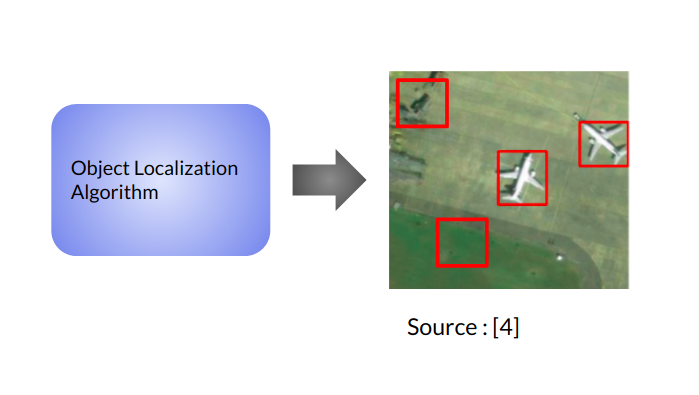
\includegraphics[height=50mm,width=92mm]{img/fig1.png}}
\caption{Example of object localization}
\label{fig1}
\end{figure}

The red colored bounding boxes are the potential object proposals. These bounding boxes will be used for fetaure extraction.

\section{Sliding Window Approach}
Sliding window technique is one of the traditional approach for object localization. In this technique, we define a window of certain height and width which will be sliding throughout the image with a certain stride length. Each of these windows will be provided to the feature extraction module and based on the features it will be classified as object window or non-object window. Working of this approach is described in figure \ref{fig2}. In figure \ref{fig2} each block is a window and the stride length of sliding is 1.

\begin{figure}[!htbp]
\centerline{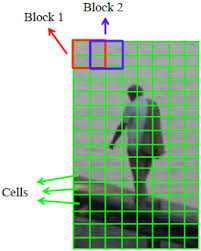
\includegraphics[height=50mm,width=50mm]{img/fig2.jpeg}}
\caption{Sliding window approach, source: https://stackoverflow.com}
\label{fig2}
\end{figure}



\par This approach has many drawbacks, such as it is computationally intensive and the window might not contain the whole object etc. 


\section{Ellipse and Line Segment Detector (ELSD)}
ELSD \cite{b4} can detect rectangular and curved region in an image. It is can be used on any gray-scale images without performing any edge-detection algorithm on the image. It acts as a geometric shape detector. It is used for candidate selection in satellite images because many times the object of interest is circular or ellipsoidal in shape, e.g, wells, oil-tanks etc. ELSD can be carried out in two steps: 
\begin{itemize}
    \item \textbf{Candidate selection: }This is done by performing the process of region growing. Here, we start from a seed pixel and then pixels were grouped into connected regions based on their gradient orientation. The gradient of a pixel can be defined as the direction of change of intensity in the image. 
    \par By region growing and region chaining operation we can get chains of rectangular regions. Now, there are two constraints that will enforce the chain of rectangular regions to be \textit{convex} and \textit{roughly smooth}.
    \par First one is \textbf{convexity constraint}. In this constraint two consecutive rectangular regions should have same directional change in gradient, i.e, $\Delta \theta_i$ and $\Delta \theta_{i+1}$ should have the same sign, given in figure \ref{fig3}.
    \par Second one is the \textbf{roughly smooth constraint}. That is, the change in gradient in two consecutive rectangular region should not exceed the value of $\pi / 2$. This curve growing procedure produce a ``polygonal approximation" \cite{b4} like circular and elliptical shapes. Hence, at the end of this step we get three types of candidates: i) rectangular regions, ii) circular regions and iii) elliptical regions. 
    
    \begin{figure}[!htbp]
    \centerline{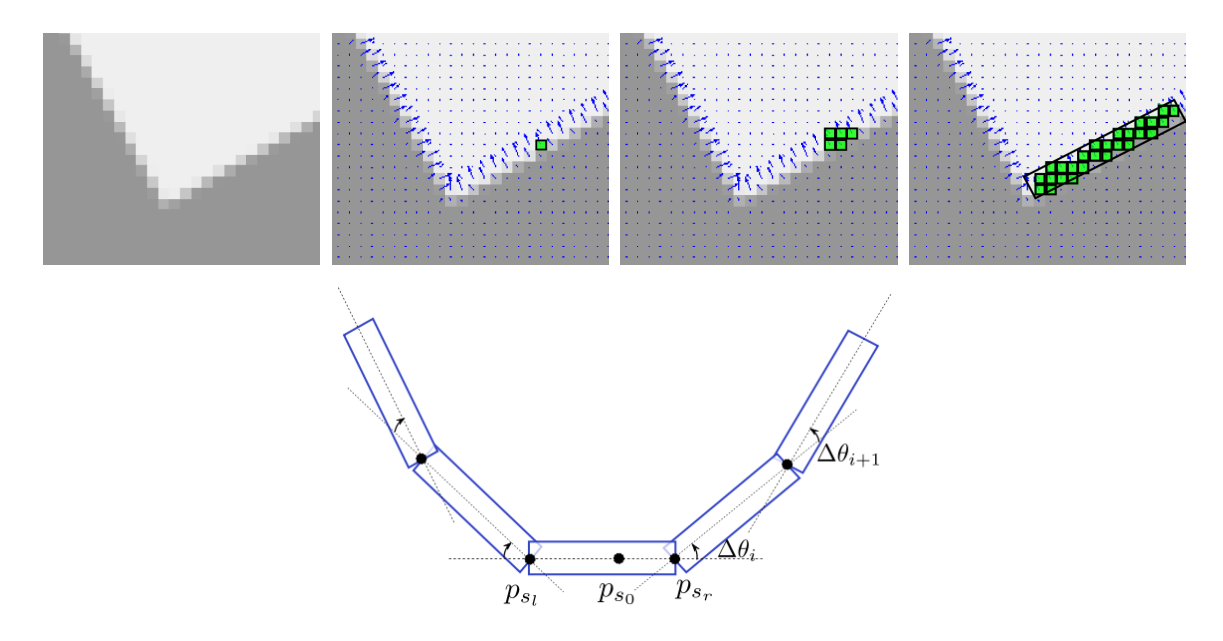
\includegraphics[height=90mm,width=150mm]{img/fig3.png}}
    \caption{Region growing and curve growing. Source: \cite{b4}}
    \label{fig3}
    \end{figure}
    
    \item \textbf{Validation: }It is the process in which we validate the candidates, i.e, it is checked that the candidates have elliptical, circular shape or not. Here, we calculate the number of aligned pixels for each region. The criteria for alignment of a pixel in a curved region is given as: $$Angle(\Delta x(p),\ dir_{\perp}(tan_c(p))\leq \sigma \pi$$ where $\Delta x(p)$ is the gradient of the image $x$ at pixel $p$ and $dir_{\perp}(tan_c(p))$ is the direction orthogonal to the tangent $tan_c(p)$ of the circle or ellipse $c$ at pixel $p$. Here $\sigma$ is the precision value and generally it is set as $1/8$. Some examples of aligned pixels is given in figure \ref{fig4}.
    
    \begin{figure}[!htbp]
    \centerline{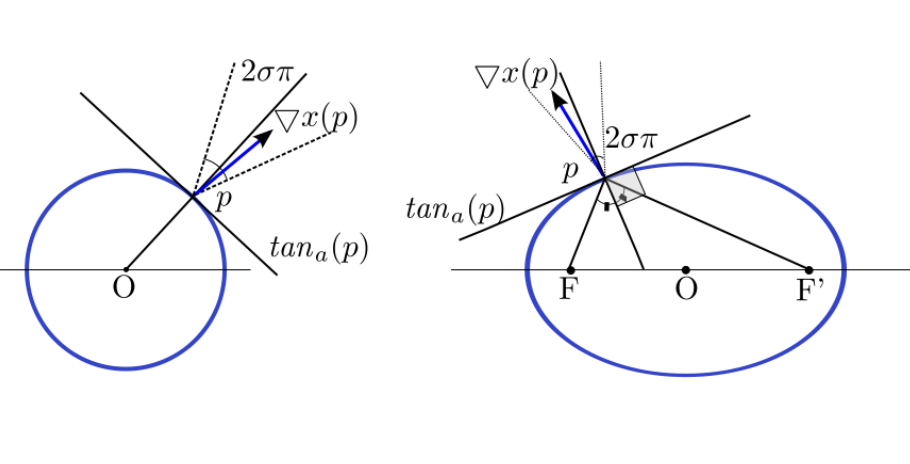
\includegraphics[height=50mm,width=90mm]{img/fig4.png}}
    \caption{``Segments $s$ containing $\sigma$-aligned pixels". Source: \cite{b4}}
    \label{fig4}
    \end{figure}
    
    If the number of aligned pixel for the candidate is greater than a threshold then it is validated as a circular or elliptical shaped region. 
    
\end{itemize}

\par ELSD produces all the elliptical and circular connected regions as output but these regions might not contain our object of interest. Especially, if the object is not circular in shape, e.g, air-crafts. 

\subsection{Modified ELSD}
Zhang et. al. \cite{b6} has modified the traditional ELSD algorithm, specifically for oil-tank detection purpose. As we know that oil-tanks are generally circular in shape and they can not have more radius than a threshold. Hence, alongwith number of aligned pixels constraint they have used another constraint as described below: $$| \sqrt{(cir_r-cen_r)^2+(cir_c-cen_c)^2}-R|\leq \eta,\ and\ \eta \geq 0$$
where $cir_r$ and $cir_c$ are the row and column position of the pixel on the circle respectively and $cen_r$ and $cen_c$ are the row and column position of the center of the circle respectively. $R$ is the radius of the circle and $\eta$ is the threshold for controlling the size of the circular region. Based on these two constraints the candidate regions have been proposed.


\section{Binarized Normed Gradients (BING)}
BING \cite{b2} is an algorithm which can produce potential object windows from an image. It calculates the objectness score for each window and based on that it selects some of the windows if they are above a threshold value. Cheng et. al. \cite{b2} observed that the small image windows of fixed size within an object shares a significant correlation with each other. Thus each image window is re-sized to a fixed size (e.g, $8\times 8$) window. For objectness score calculation, the norm of gradients of each pixel in the $8\times 8$ window is calculated and represented as a 64-dimensional feature vector which will be provided to a cascaded SVM classifier for classification. This 64D feature vector is called normed gradients (NG) feature. If this 64-dimensional feature vector is calculated for binarized version of $8\times 8$ window then this feature will be called binarized normed gradient (BING) feature. 
\par A fixed size window is scanned over the image to find any generic object that are present in it. Each such window will get a score, which will be calculated as: 
$$s_l=W\cdot g_l,\ l=(i,x,y)$$ where $s_l$ is the filter score, $g_l$ is the normed gradient feature, $l$ is the location, $i$ is the size, $W\in \R^{64}$ is the weight vector that has been assigned as co-efficient of filter score for each window, $W$ is learned by a linear SVM model and $(x,y)$ is the position of the window. For each i, a small number of proposals will be selected using non-max suppression. Non-max suppression is an algorithm which eliminates the similar bounding boxes or windows based on a threshold value of overlapping between two windows. Based on the filter score $s_l$, the actual objectness score is calculated using the formula $$o_l=v_i\cdot s_l+t_i$$ where $o_l$ is the objectness score of the window at location $l$, $v_i,\ t_i$ are the co-efficient and a bias term which can be learned with an SVM classifier respectively. Normed gradient features of some object windows and non-object windows are used as ground truth positive and negative samples respectively for training.  

\par Wu et.al. \cite{b5} has used this objectness score to detect potential windows containing air-craft. They have imposed some constraints on the output windows for filtering. The constraints are: 
\begin{itemize}
    \item Windows with high height/width ratio has been chosen where ratio is $$ratio=\frac{max(height, width)}{min(height,width)}$$. If the ratio is above a certain threshold then the window is chosen.
    
    \item Windows, that has area under a certain range $[A_i,A_j]$ is chosen where area of the window is calculated as $$area=height\times width$$.
    
    \item Windows that has objectness score $o_l$ which is above a threshold  value $o_t$ is chosen.
\end{itemize}
\par The result of applying BING on satellite images containing air-crafts is given in figure \ref{fig5}.

\begin{figure}[!htbp]
\centerline{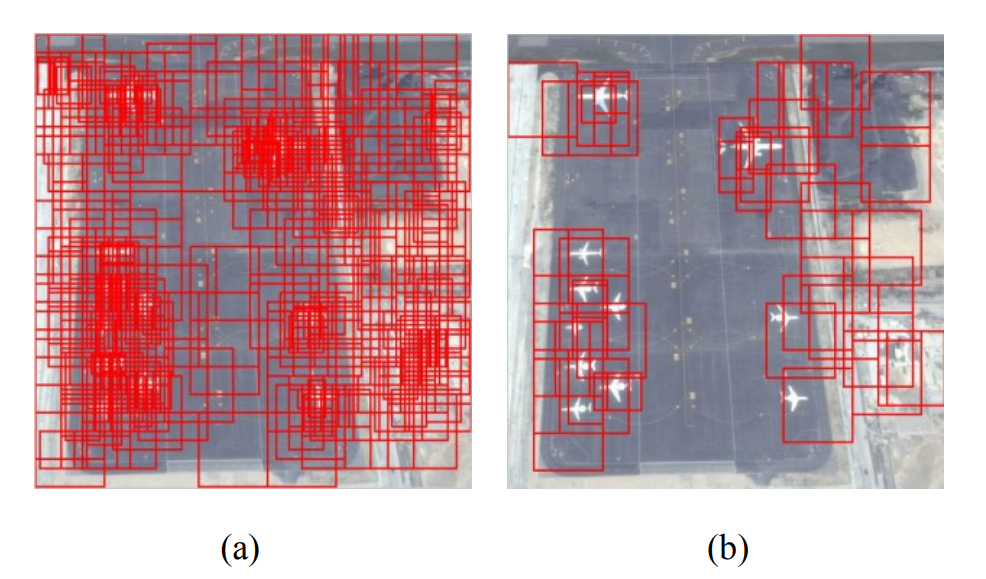
\includegraphics[height=60mm,width=100mm]{img/fig5.png}}
\caption{(a) Bounding boxes proposed by BING. (b) Bounding boxes after imposing the constraints. Source: \cite{b5}}
\label{fig5}
\end{figure}

\chapter{Feature Extraction}
Feature extraction is the process of collecting relevant information from each data sample (object windows), which will be unique based on the class of the data sample. Features define each object uniquely in a satellite image. Features can help to differentiate between the objects and non-objects. We extract features from the potential object windows to predict if the window contains the object or not. 
\par In this survey, we have only focused on deep learning based feature extraction techniques, e.g, CNN.


\section{Convolutional Neural Networks (CNN)}
Convolutional neural networks is a type of feed-forward neural network which is specifically designed for features extraction from images. CNN has two types of layers, using which it can perform the forward and backward propagation. 
\par Forward propagation is performed by doing convolution operation on the pixels of the image with different number of filters and apply a non-linear activation function (e.g, ReLu) on the result along with a bias term. Here, the filters act as weight for the images. The result is given in figure \ref{fig6}.

\begin{figure}[!htbp]
\centerline{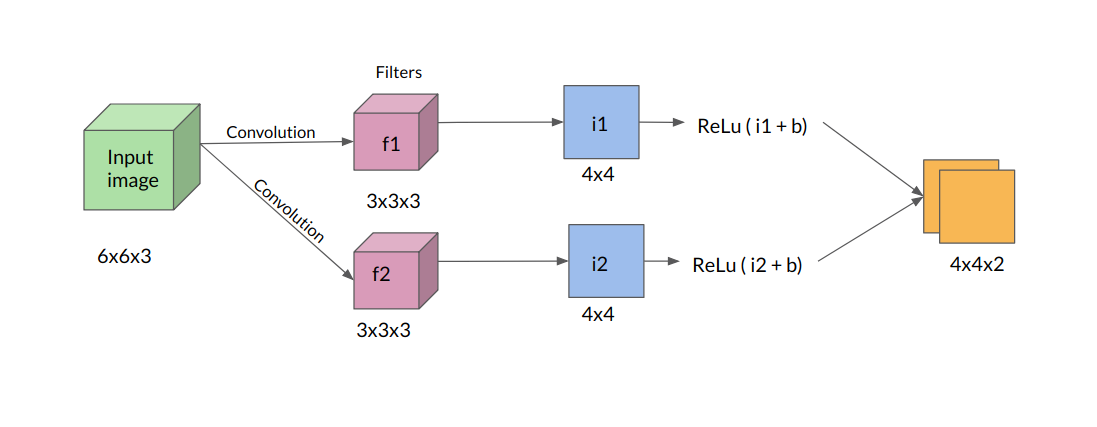
\includegraphics[height=80mm,width=160mm]{img/fig6.png}}
\caption{Result of one layer of convolution operation}
\label{fig6}
\end{figure}

\par The result from each filter is clubbed together and forwarded to the pooling layer. Pooling layers will reduce the size of the feature representation and speed up the computation. There are several kinds of pooling layers, e.g, max-pooling, average pooling etc. In max-pooling we apply filter on the input which will perform max operation. It is similar to previous step, only difference is that, instead of convolution we perform max operation. Example of max pooling is given in figure \ref{fig7}. 

\begin{figure}[!htbp]
\centerline{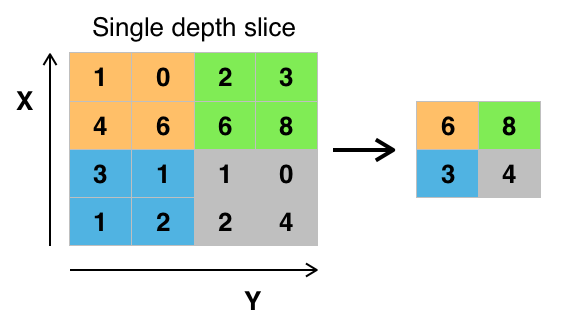
\includegraphics[height=50mm,width=85mm]{img/fig7.png}}
\caption{Result of max-pooling operation. Source: https://en.wikipedia.org}
\label{fig7}
\end{figure}

In average pooling we perform the averaging operation on the input. The general architecture of the CNN is given in figure \ref{fig8}.

\begin{figure}[!htbp]
\centerline{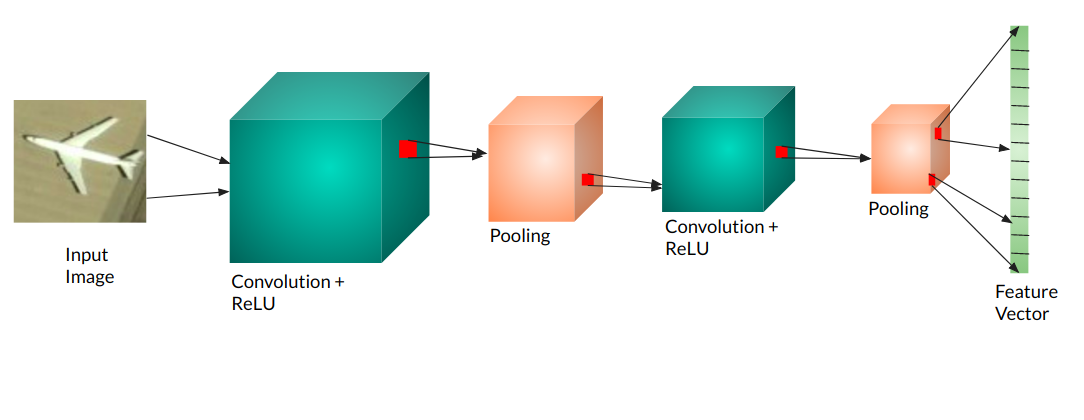
\includegraphics[height=60mm,width=150mm]{img/fig8.png}}
\caption{General architecture of a CNN}
\label{fig8}
\end{figure}

At the last layer we will get a volume of specific size as output. Let the size of this volume is $m\times n\times p$. Then this volume will be flattened to a vector of feature of dimension $[m\times n\times p, 1]$. This feature vector will be forwarded to the classification stage.

\par Wu et.al. \cite{b5} has used CNN architecture for feature extraction. They have created a model with 4 layers. The architecture is C-S-C-S, where C is convolutional layer and S is pooling layer. $32\times 32$ sized images has been given as input to the architecture. The filter size at convolutional layer is $5\times 5$ and size of pooling filter is $2\times 2$.


\section{CNN with Histogram Oriented Gradients (HOG)}
Zhang et.al \cite{b6} has used this combined method for feature extraction. They have done oil-tank detection in satellite images. It has been observed that the surrounding of an oil-tank consists of shadows, trees, pipelines and other oil-tanks. So, the authors has used CNN to extract this surrounding feature and HOG to extract the local feature of the oil-tank. Local feature means the feature of the oil-tank only. As there could be many oil-tank like circular objects present in satellite images, thus the authors has used both these features to correctly detect and localize the oil-tanks. 
\par We have already discussed about CNN in the above section, thus in this section we will describe the HOG feature calculation process.
\subsection{Histogram Oriented Gradients (HOG)}
HOG can accurately represent the information about the shape of an object present in an image. The main idea behind HOG is that the distribution of gradient orientation has the capacity to accurately detect and characterize the appearance of the objects. 
\par Feature descriptor of an image fetches out the important information and eliminates the excess informations. It converts the image into a flat vector of features. HOG \cite{b7} feature descriptor takes $64\times 128$ images as input. First the input is pre-processed by performing gamma correction. 
\par Then, the horizontal and vertical gradients are calculated using filters. The filtering is done by using horizontal and vertical kernel shown in figure \ref{fig9}.

\begin{figure}[!htbp]
\centerline{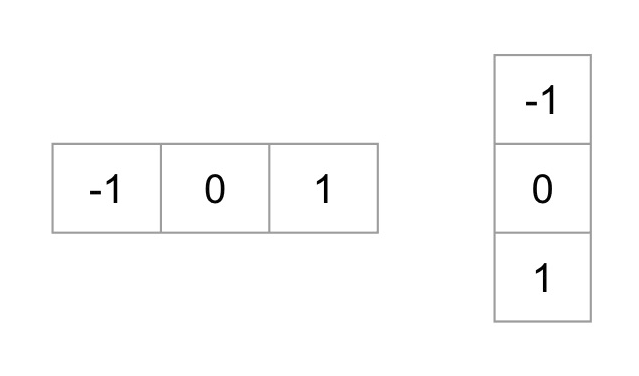
\includegraphics[height=60mm,width=120mm]{img/fig9.png}}
\caption{Horizontal and vertical kernels. Source: https://www.learnopencv.com}
\label{fig9}
\end{figure}

By using horizontal and vertical gradients we can calculate the modulus and direction of the gradient using the formula:
$$g=\sqrt{(g_x)^2+(g_y)^2},\ \theta=tan^{-1}(\frac{g_y}{g_x})$$ where $g_x$ is the horizontal gradient and $g_y$ is the vertical gradient. $g$ is the gradient modulus and $\theta$ is the gradient direction.

\par Now we divide the images into cells of size $8\times 8\times 3$ pixels, where $3$ is the number of channels, i.e, R,G, B. We calculate the gradient for each of these cells using the process described above. After gradient calculation, the cell is converted to size $8\times 8\times 2=128$ values. This is depicted in figure \ref{fig10}. 

\begin{figure}[!htbp]
\centerline{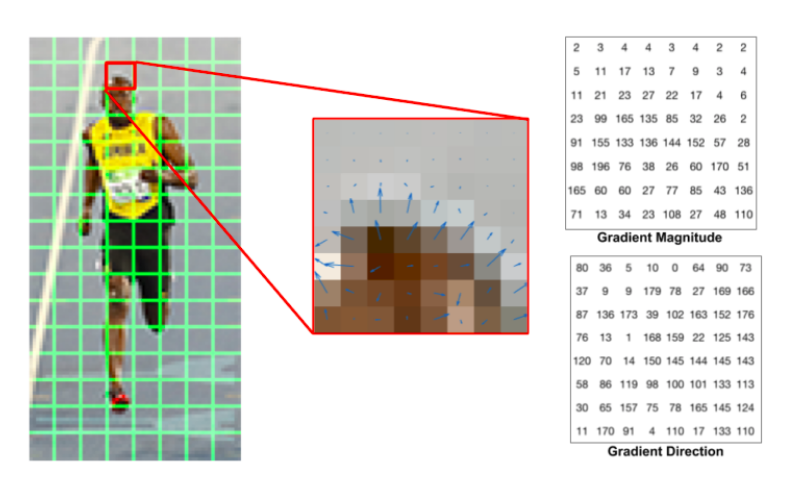
\includegraphics[height=90mm,width=150mm]{img/fig10.png}}
\caption{Conversion of cells into gradients. Source: https://www.learnopencv.com}
\label{fig10}
\end{figure}

These 128 values are represented using a 9-bin histogram. The 9-bin histogram is an array of 9-numbers corresponding to angles 0, 20, 40, 60,..., 160. Now, based on the gradient direction matrix we put the corresponding values from gradient modulus matrix to a particular position of the 9-bin histogram array. This mapping is depicted in figure \ref{fig11}.

\begin{figure}[!htbp]
\centerline{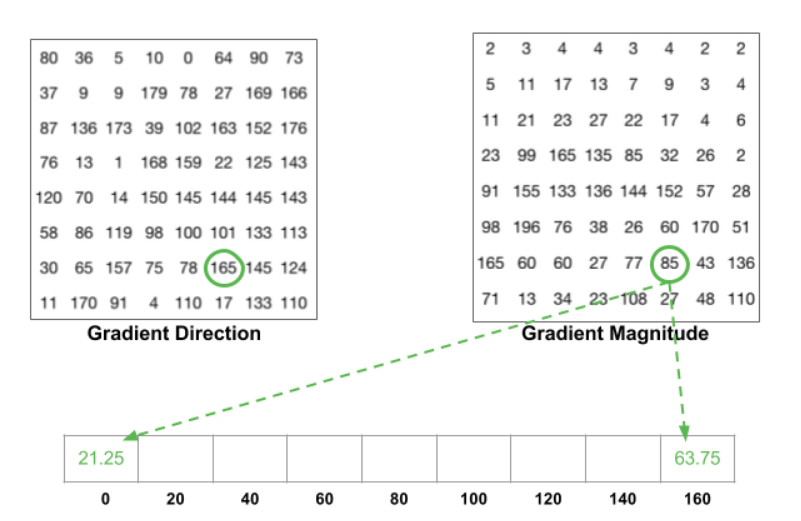
\includegraphics[height=60mm,width=120mm]{img/fig11.png}}
\caption{Mapping into 9-bin histogram array. Source: https://www.learnopencv.com}
\label{fig11}
\end{figure}

In the next step, we perform the block normalization. We take $16\times 16$ block, consisting of 4 cells. We calculate 9-bin histogram for each of the cell and concatenate all of them together which will produce a vector of dimension $36\times 1$. Now, to make the procedure more robust to lightning, we perform normalization on this $36\times 1$ vector by dividing each of its element with the L2 norm of the vector. For each $16\times 16$ block we calculate this vector and finally we concatenate them all together to get the HOG feature.


\section{Hybrid Deep Convolutional Neural Networks (HDNN)}
Deep convolutional neural networks is basically a CNN with a multi-layer perceptron (MLP) classifier. The CNN acts as a feature extractor and the MLP acts as a classifier. Here, CNN extracts feature of only one scale, i.e, it is not able to detect the ``large scale variance" \cite{b8} of objects. The objects show ``large scale variance" when they appear big in some images and small in some other images. CNN might not be able to detect this scale variance. 
\par Now, in this scenario HDNN \cite{b8} comes into the picture. Before describing the architecture of HDNN, let us introduce two definitions : 
\begin{itemize}
    \item \textbf{Source area: } Source area of a pixel in the output feature block is defined as the number of pixels from the input image that has been gone through each filter and resulted in that pixel in the output feature block. 
    \item \textbf{Feature scale: }It is the largest source area of a pixel in the output feature block from a CNN. 
\end{itemize}
\par Chen et.al \cite{b8} has used $7\times 7$ filters in convolution layer 1, $4\times 4$ filters in convolution layer 2 and also $4\times 4$ filters in convolution layer 3. Hence, the maximum source area of a pixel in the output feature block can be $28\times 28$. So, for each $28\times 28$ patch in the input image we will get one pixel in the output feature block. This shows that traditional CNN only extracts same scaled features. 
\par On the other hand, HDNN divides the last layer of convolution and pooling layers into $n_b$ number of blocks. Each block will be connected to the previous pooling layer. Each of the block has different filter size and max-pooling field size. Chen et. al \cite{b8} has divided the last layer into three blocks. First and second block has filter of size $4\times 4$. Thus the source area of the pixel of the feature block that will be resulted by these two blocks will be $28\times 28$. Whereas the third block has filter size $6\times 6$, which can indicate that the largest source area or feature scale of a pixel in the output feature block will be $36\times 36$. Hence, HDNN can extract features of different scales from the input images. The architecture of the HDNN is given in figure \ref{fig12}.

\begin{figure}[!htbp]
\centerline{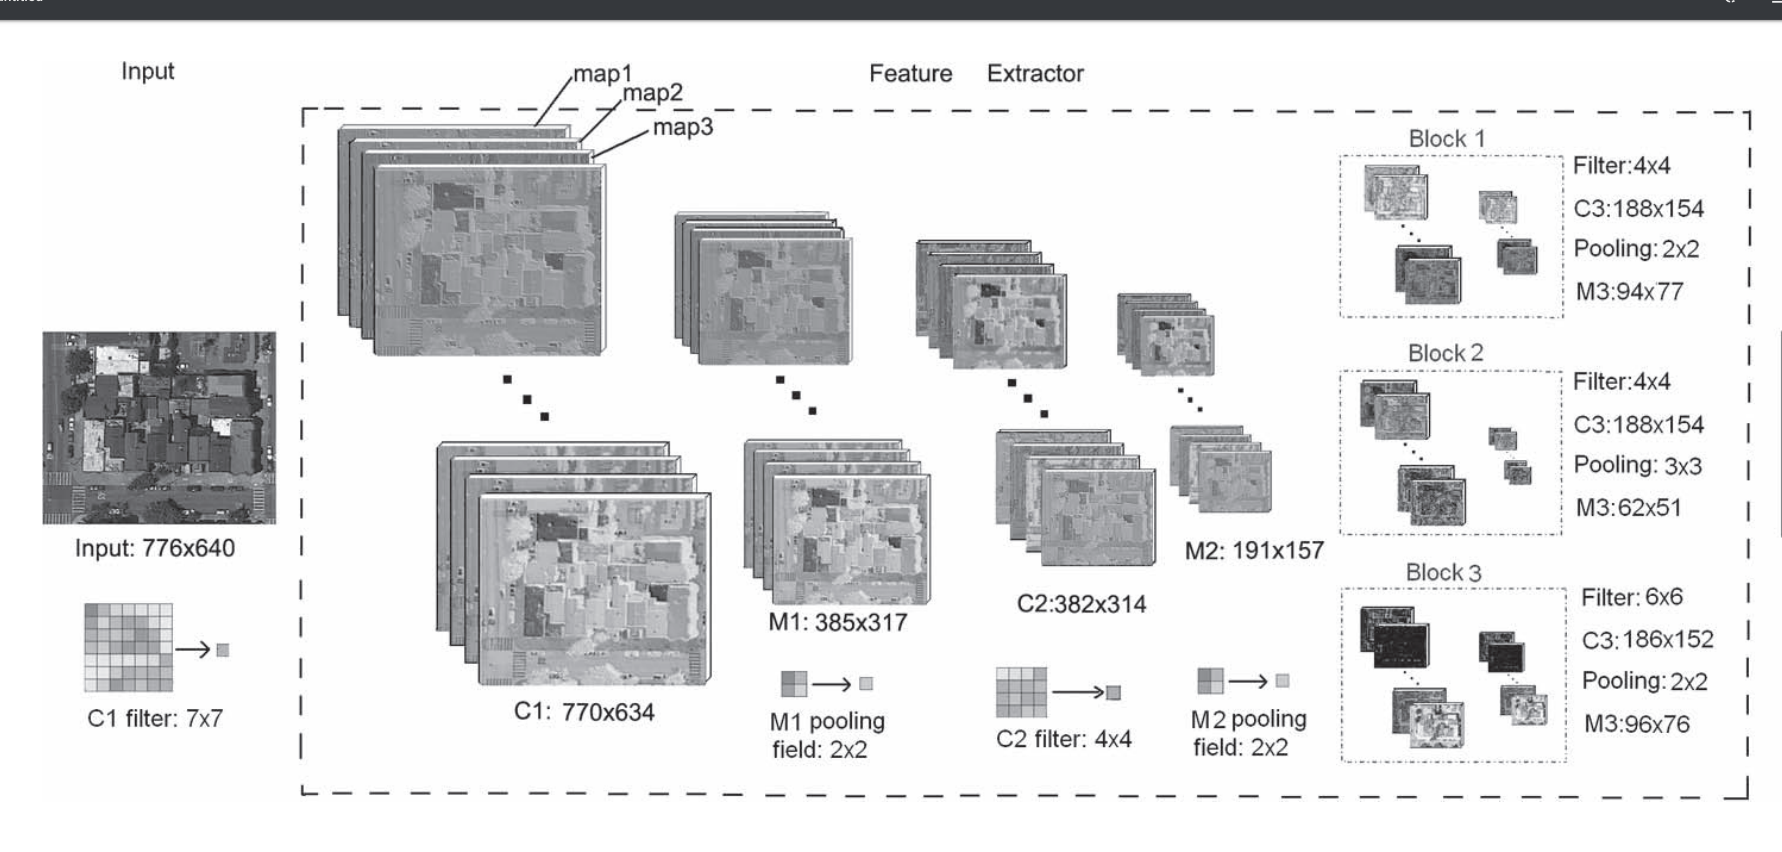
\includegraphics[height=80mm,width=140mm]{img/fig12.png}}
\caption{Architecture of HDNN. Source: \cite{b8}}
\label{fig12}
\end{figure}

\par These blocks having different filter sizes are responsible for producing the variable scaled feature vector of the object. 
\chapter{Classification}
Classification is the final step for object detection in satellite images. Based on the extracted features from the images we classify them using some standard classifier, e.g, support vector machines (SVM), MLP etc. The classifier learns the patterns from the features of an image and predicts the label of that image.

\section{Support Vector Machine (SVM)}
SVM \cite{b3} is used to classify two classes by finding the best hyper-plane between those two classes. The data points that are closest to the hyper-plane from the two classes are called support vectors. SVM maximizes the distance between the support vectors belonging from two different classes. The equation of the hyper-plane can be written as: 
$$\vec{w}\cdot \vec{u}+b=0$$ where $\vec{w}$ and $b$ are the weight vector and bias respectively. $\vec{w}$ is perpendicular to the hyper-plane. Now, the decision rule for SVM can be defined as:
$$\vec{w}\cdot \vec{u}+b\geq +1,\ then\ positive\ class$$ , $$\vec{w}\cdot \vec{u}+b\leq -1,\ then\ negative\ class$$
Support vectors from positive and negative class will satisfy the equation \ref{eq1} and \ref{eq2} respectively.
\begin{equation}
    \vec{w}\cdot \vec{u}+b=+1
    \label{eq1}
\end{equation}
\begin{equation}
    \vec{w}\cdot \vec{u}+b=-1
    \label{eq2}
\end{equation}
One example of SVM is given in figure \ref{fig13}.

\begin{figure}[!htbp]
\centerline{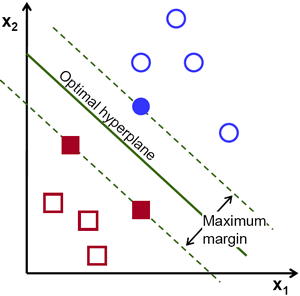
\includegraphics[height=60mm,width=60mm]{img/fig13.png}}
\caption{Working of SVM. Source:https://docs.opencv.org/}
\label{fig13}
\end{figure}

Now, we can find out the distance between support vectors from two class and maximize that distance with respect to $\vec{w}$ and $b$. 

\par The authors of \cite{b6} has used linear SVM to classify between oil-tank and non oil-tank images. The features were extracted using HOG and CNN. These feature vectors will be represented as data points as described above. 


\section{Multi-layer Perceptron (MLP)}
\par Chen et.al. \cite{b8} and Wu et.al. \cite{b5} has used MLP for classification. Multi-layer perceptron is a classifier based on the concept of artificial neural networks. It has feed-forward architecture, where the input is propagated through each computational layer. MLP has atleast three layers:
\begin{itemize}
    \item \textbf{Input layer: } In this layer we provide the extracted feature as input through various neurons. If a feature vector has 10 components then the input layer will have 10 neurons. In each neuron we will feed one component of the feature vector as input.
    \item \textbf{Hidden layer: }There could be many hidden layers in a MLP. A hidden layer can have any number of nodes. In each node, outputs of all the neurons from previous layer will be multiplied with a weight vector and then a bias will be added to it. The result of this operation will be passed to a non-linear activation function which will produce either 0 or 1. This whole operation happen in each node of the hidden layer.
    \item \textbf{Output layer: }The number of nodes in this layer depends on the type of classification. If we are doing binary classification then there will be only one node. In this node the same operation will happen as that of the hidden layer node. And it will output the label of the input as either 0 or 1. 
\end{itemize}
The structure of a multi-layer perceptron is given in figure \ref{fig14}.

\begin{figure}[!htbp]
\centerline{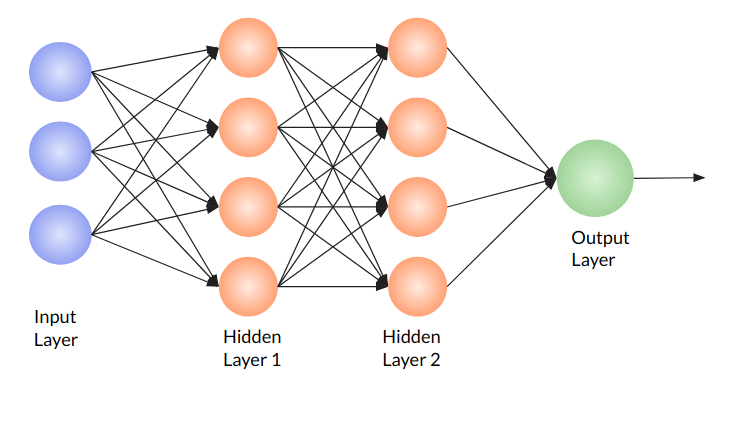
\includegraphics[height=60mm,width=110mm]{img/fig14.png}}
\caption{Architecture of MLP}
\label{fig14}
\end{figure}

\par MLP works using two algorithms:
\begin{itemize}
    \item \textbf{Forward propagation: }Here, we introduce weights and bias in each hidden layer. The computation in each node will be given as: 
    $$y_i=\sum_{n=1}^{K}w_i\cdot x_i+b,\ and$$
    $$z_i=g(y_i)$$
    where $g$ is the non-linear activation function. This function outputs value within 0 and 1 or within -1 and +1, e.g, \textit{sigmoid} function outputs in the range 0 and 1, while \textit{tanh} function outputs in the range of -1 to +1.
    \par This process will continue until the output layer is reached, which will output a label, i.e, either 0 or 1. Based on the predicted value we calculate the loss using any loss function, e.g, cross-entropy loss. We give all the images and get an output label for each of the images along with their loss. The summation of all the loss function is known as cost function. In backpropagation algorithm we minimize this cost function.
    \item \textbf{Backward propagation: }Here, we differentiate the cost function w.r.t weight vector and bias of the previous layer and we update its weight and bias by using the formula: $w_i=w_i-\Delta w_i$ and $b_i=b_i-\Delta b_i$. We keep on updating the weights in each layer and move backwards. When we reach the input layer, we again perform the forward propagation with the updated weights. 
\end{itemize}




\chapter{Evaluation}
\label{ch5}


\section{Sliding Window - HDNN - MLP}
Chen et.al. \cite{b8} has used sliding window technique with to localize the object (vehicle) in the input image. Fetaure extraction from each localized window is done using hybrid deep convolutional neural network (HDNN). Finally, classification of the extracted feature has been done using multi-layer perceptron (MLP). 

\subsection{Dataset Description}
The authors have collected 63 images of San Francisco city, having resolution $1368\times 972$ from Google earth. Out of these, 31 images are used for training, in which there were 3901 vehicles present. And rest of the 32 images were used for testing, in which 2870 vehicles were present. 
\subsection{Results}
Accuracy metrics used here are: 

\begin{figure}[!htbp]
\centerline{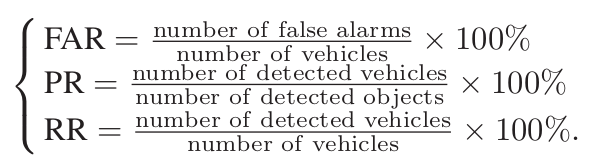
\includegraphics[height=25mm,width=90mm]{img/fig15.png}}
\caption{FAR=False Alarm Rate, PR=Precision Rate, RR=Recall Rate. Source: \cite{b8}}
\label{fig15}
\end{figure}

The authors have experimented with the blocks of different feature scale in HDNN and they have found out that an architecture of blocks with feature scale 44-20-20 works the best with 95\% recall and only 12.8\% false alarm rate. Here, 44 means that the first block has feature scale $44\times 44$, similar for 20 also. The results are shown in figure \ref{fig16}. They have also compared the precision and recall rate of differently architectured HDNN and traditional deep convolutional neural network (DNN). The results of the comparison of precision and recall rate is given in the figure \ref{fig17}.  

\begin{figure}[!htbp]
\centerline{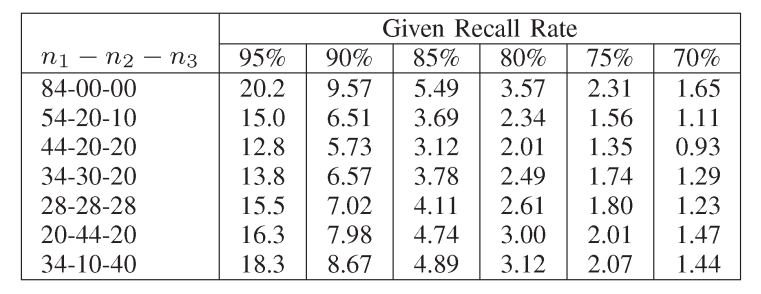
\includegraphics[height=30mm,width=90mm]{img/fig16.png}}
\caption{Relation between architecture of HDNN and FAR. Source: \cite{b8}}
\label{fig16}
\end{figure}

\begin{figure}[!htbp]
\centerline{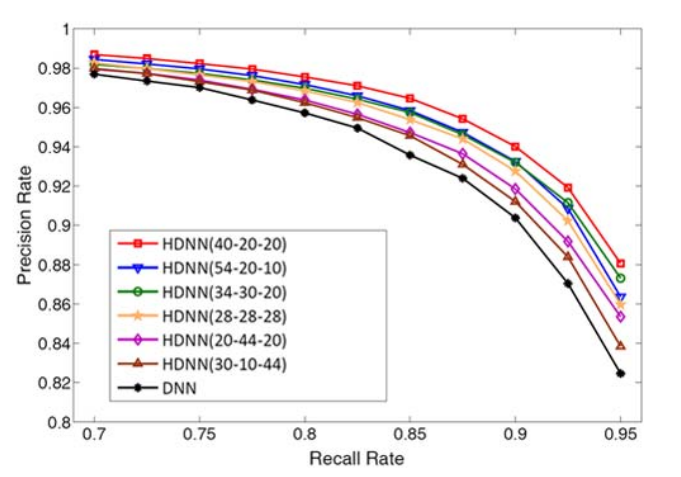
\includegraphics[height=60mm,width=80mm]{img/fig17.png}}
\caption{``Recall precision curves of HDNNs and DNN". Source: \cite{b8}}
\label{fig17}
\end{figure}


\section{ELSD - CNN and HOG - SVM}

\subsection{Dataset Description}
The authors have collected 54 images from Google Earth. 42 images has been used for training and parameter selection in ELSD while other images were used for testing purposes. By applying ELSD on 42 training samples, they have got 4264 positive samples and 7119 negative samples. They have also done data augmentation by rotating the images in every \ang{45} for more generality. After data augmentation, the number of positive and negative samples were 34112 and 56952 respectively. The test dataset contains 12 images of size $3712\times 3008$ pixels.

\subsection{Results}
Zhang et.al.\cite{b6} has used ellipse and line segment detector (ELSD) for candidate selection, CNN and HOG for feature extraction and linear SVM for classification. 
\par The authors have experimented with different values of circle threshold $\eta$ in their modified ELSD method. The results are given below: 

\begin{figure}[!htbp]
\centerline{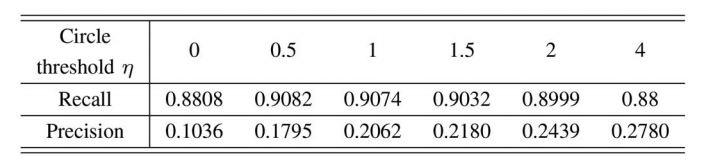
\includegraphics[height=20mm,width=90mm]{img/fig18.png}}
\caption{Precision and recall for certain values of $\eta$. Source: \cite{b6}}
\label{fig18}
\end{figure}

The modified ELSD method has achieved \textbf{90.74\%} recall rate with \textbf{26.12\%} precision rate. And linear SVM with HOG-CNN as feature vector has achieved \textbf{91.84\%} recall rate and \textbf{97.51\%} precision rate. The result of applying HOG-CNN on test images is depicted in the figure \ref{fig19}

\begin{figure}[!htbp]
\centerline{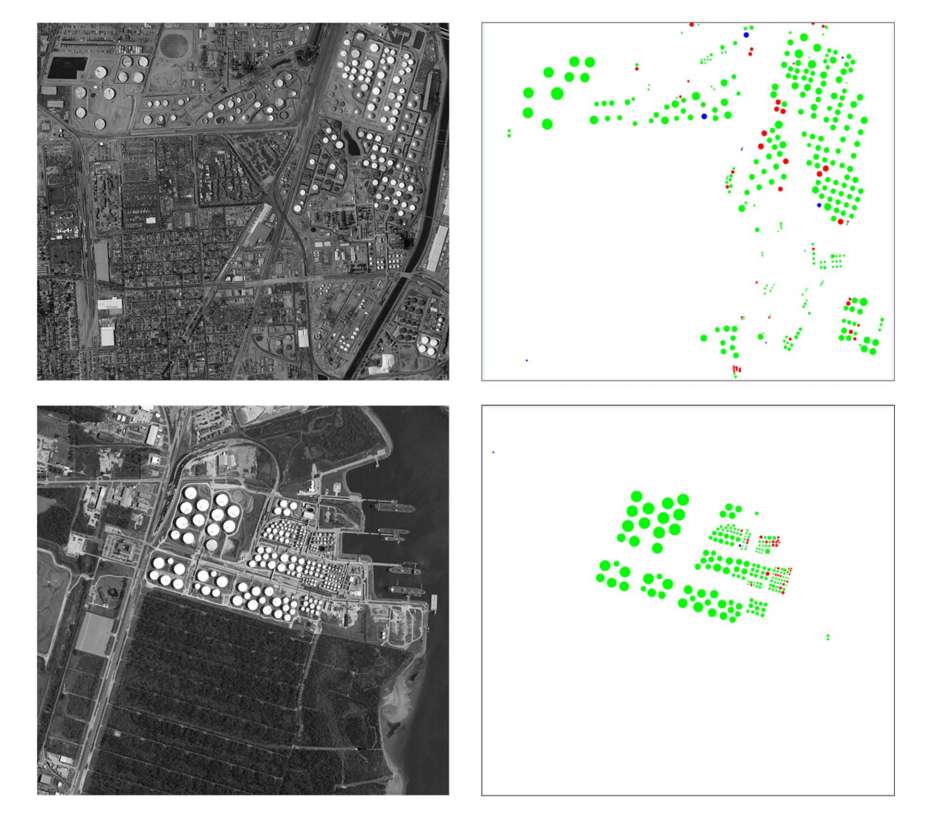
\includegraphics[height=130mm,width=150mm]{img/fig19.png}}
\caption{Examples of applying HOG-CNN. Source: \cite{b6}}
\label{fig19}
\end{figure}



\section{BING - CNN - MLP}
In this paper \cite{b5}, the authors has used binarized normed gradients for object localization, CNN for feature extraction and MLP for classification. 
\subsection{Dataset Description}
The authors have collected 500 positive image patches of aircraft and 5000 negative image patches from Google Earth. Then the 500 positive image patches were augmented by rotation of \ang{90} for 4 times, which resulted into 2000 image patches. 
\par The test dataset has 26 images of varying sizes of $565\times 369$ to $1484\times 865$.

\subsection{Results}
Here also the false alarm rate, precision rate and recall rate has been used as accuracy metrics. They are described in the figure \ref{fig15}. 
\par The authors have achieved \textbf{90.05\%} of precision rate with \textbf{80\%} of recall rate. And also the false alarm rate is \textbf{17.66\%} with \textbf{85\%} of recall rate. The variation of false alarm rate with recall rate is given below:\\ \\
\begin{tabu} to 0.9\textwidth { | X[l] | X[c] | }
 \hline
 \textbf{False Alarm Rate} & \textbf{Recall Rate} \\
 \hline
 3.75\%  & 65\%\\
\hline
4.42\% & 70\%\\
\hline
7.28\% & 75\%\\
\hline
9.27\% & 80\%\\
\hline
17.66\% & 85\%\\
\hline
\end{tabu}
\\ \\
The results of applying BING-CNN on test images is depicted in figure \ref{fig20}.

\begin{figure}[!htbp]
\centerline{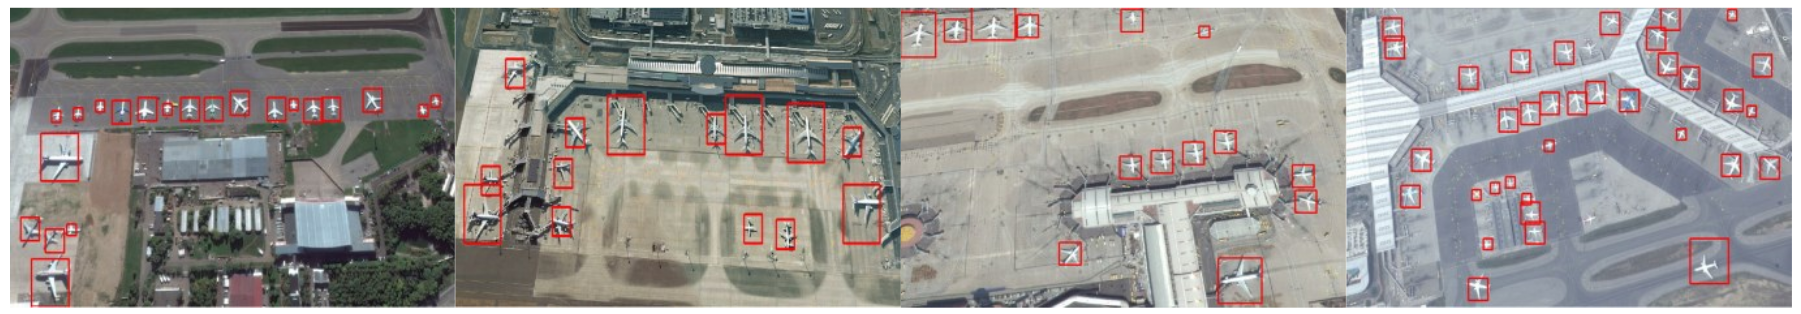
\includegraphics[height=50mm,width=160mm]{img/fig20.png}}
\caption{Examples of applying BING-CNN. Source: \cite{b5}}
\label{fig20}
\end{figure}

\par Wu .et.al.\cite{b5} have not evaluated the performance of BING on their dataset. So, the performance of BING \cite{b2} in VOC2007 test set has been described. This dataset contains 4952 images with bounding box annotations. There are 20 different classes present in the dataset. BING has achieved \textbf{99.5\%} detection rate with 5000 object proposals. Detection rate can be defined as the number of objects that are correctly detected, divided by total number of objects.



\chapter{Experimental Study}
Apart from surveying the literature, I have also done some experimental studies, like collecting data, implementing CNN followed by fully connected neural network and deploying this model on my collected data. 

\section{Problem Statement}
We need to detect wells present in satellite images of some specific villages of Maharashtra. The main motivation to solve this problem is to tackle the problem of water deprivation. By detecting wells and water-bodies in a region we can find out the villages which does not have enough water resources.
\par This is a problem of binary classification, where given an image we can classify it as either an image of well or non-well.


\section{Dataset Preparation}
I have prepared a dataset of ground truth images of well and non well images. I have manually collected the co-ordinates of the wells and downloaded the image of that co-ordinate from Google Earth. I have collected around 769 well images and 700 non-well images of size $64\times 64$. 
\par For training the model, 500 well images and 500 non-well images are used. And for testing the model 269 well images and 200 non-well images has been used. 


\section{Methodology}
I have used CNN as feature extractor and MLP as classifier in my model. I have created a two layered convolutional neural network model. The description of the model is given as: 
\begin{itemize}
    \item The first convolutional stage is with ReLU activation function followed by a max-pooling layer. This layer has 20 convolutional filters, each one of them has a size of $5\times 5$. The output dimension is same as that of the input shape i.e, $64\times 64$. As this is the first layer in our model, we have to define its input shape i.e, (1,64,64). The max-pooling operation applies a sliding window that slides over the image and takes the maximum value of pixel present in that region.
    
    \item The second convolutional layer is also followed by ReLU activation function and a max-pooling layer. Now, we increase the number of convolutional filters to 50 from 20 in the previous layer.
    
    \item Then we have a standard flattening layer and a dense layer of 500 neurons. This flattening layer flattens the last 3D feature block of the CNN and provides it to the dense layer. This dense layer acts as a hidden layer. The output layer of the MLP has softmax function as activation function, which can be defined as: $$P(y=j|X)=\frac{e^{X^T\cdot w}}{\sum_{k=1}^{K}e^{X^T\cdot w}}$$ where $K$ is the number of classes and $P(y=j|X)$ is the probability of the input being in class $j$ given it's feature vector $X$.
\end{itemize}

\subsection{Brief Description of the Hyper-parameters}
The parameters to the CNN model are the filters and biases. But there are some other indirect parameters which control these primary parameters. These are called the hyper-parameters. 
\begin{itemize}
    \item \textbf{Learning rate: }It is the rate at which the weight updation happens during back-propagation algorithm. If it is very small then weight updation will be slow which will result in slow convergence of the back-propagation algorithm.
    \item \textbf{Batch size: }It is the number of samples that will be propagated to the network of the model. This results in less amount of memory requirement during the training process. And training process becomes faster. But if the batch size is too small then the model will not be able calculate the gradient accurately.
    \item \textbf{Number of epochs: }Number of iterations that will be executed while doing the gradient descent. Gradient descent is an algorithm to update the weights based on the loss. More number of iterations might lead to over-fitting and the training process will be longer. On the other hand, less number of epochs might lead to under-fitting.
    \item \textbf{Optimizer: }In our model we have used Adam optimizer. This is basically an algorithm to reduce the loss by updating the weights in a proper way. This algorithm is similar to gradient descent algorithm but the only difference is variable learning rate. That is, in every iteration the learning rate varies.
    \item \textbf{Loss function: }This function calculates the amount of miss-classification done by the model. Here, I have used cross-entropy loss function. Cross-entropy loss function for binary classification is defined as: 
    $$loss=-ylog(a)-(1-y)log(1-a)$$ where $y$ is the ground truth label and $a$ is the predicted label. 
    \item \textbf{Validation split: }We train the model with certain amount of data and validate the model with the rest of the training data, e.g, in my model I have used validation split as 0.2, i,e, the model will be trained with 80\% of the training data and will be validated with the rest of the 20\% training data.
\end{itemize}
The values of various hyper-parameters of the model is described below: \\

\begin{tabu} to 0.9\textwidth { | X[l] | X[c] | }
 \hline
 \textbf{Hyper-parameter} & \textbf{Value} \\
\hline
Batch size & 128\\
\hline
Number of epochs & 50\\
\hline
Optimizer & Adam optimizer\\
\hline
Loss function & Cross-entropy loss\\
\hline
Validation split & 0.2 \\
\hline
\end{tabu}
\\

The code of the model architecture is given below: 
\begin{lstlisting}[caption=CNN model]
class LeNet:
    @staticmethod
    def build(input_shape, classes):
        model = Sequential()
        
        model.add(Conv2D(20, kernel_size=5, padding='same', input_shape=input_shape))
        model.add(Activation("relu"))
        model.add(MaxPooling2D(pool_size=(2,2),strides=(2,2)))
        
        model.add(Conv2D(50, kernel_size=5, border_mode="same"))
        model.add(Activation("relu"))
        model.add(MaxPooling2D(pool_size=(2,2), strides=(2,2)))
        
        model.add(Flatten())
        model.add(Dense(500))
        model.add(Activation("relu"))
        
        model.add(Dense(classes))
        model.add(Activation("softmax"))
        return model
\end{lstlisting}

\section{Results}
Before jumping onto the results, I want to describe the accuracy metrics. They are described below: 
\begin{itemize}
    \item \textbf{True positives (TP): }Number of samples that are correctly classified and labeled as ``well".
    \item \textbf{True negatives (TN): }Number of samples correctly classified and labeled as ``non-well".
    \item \textbf{False positives (FP): }Number of miss-classified samples that has been predicted as ``well".
    \item \textbf{False negatives (FN): }Number of miss-classified samples that has been predicted as ``non-well".
    \item \textbf{Precision: }It is defined as: $$Precision=\frac{TP}{TP+FP}$$
    \item \textbf{Recall: }It is defined as:
    $$Recall=\frac{TP}{TP+FN}$$
    \item \textbf{Accuracy: }It is defined as:
    $$Accuracy=\frac{TP+TN}{TP+TN+FP+FN}$$
\end{itemize}
The results of deploying the above mentioned trained model on 469 test images is given below:
\begin{itemize}
    \item \textbf{Test accuracy}:  0.9275053307445827
    \item \textbf{Correctly classified images}:  435
    \item \textbf{True Negatives}:  211
    \item \textbf{True Positives}:  224
    \item \textbf{False Positives}:  19
    \item \textbf{False Negatives}:  15
    \item \textbf{Precision}:  0.9218106995884774
    \item \textbf{Recall}:  0.9372384937238494
\end{itemize}

Hence, the \textbf{test accuracy} achieved by my model is \textbf{92.75\%}. The \textbf{precision rate} and \textbf{recall rate} are \textbf{92.18\%} and \textbf{93.72\%} respectively. The reason behind non-zero false positives and false negatives is the scarcity of data. We have trained the model with very less amount of images. By increasing the amount of data the accuracy will increase. I have concluded this from my previous experiments. At the very beginning I trained the model with only 132 images and tested on 100 images. The model has achieved around 82.33\% test accuracy. 
\par I have not changed the architecture of the model. Instead I increased the amount of data and the accuracy has also increased progressively. In this experiment I have not used any object localization algorithm.
\chapter{Conclusions}
\section{Comparison of Different Methods}
The first method, i.e, sliding window - HDNN - MLP has used sliding window technique for object localization,  which is a slow and computationally intensive technique. For feature extraction HDNN has been used, which can extract variable scaled features but Chen et.al.\cite{b8} have not considered the surrounding features of the air-crafts. Also they had used MLP for classification, which requires considerable amount of data for accurate classification. But, the authors did not have that much data. This might be the reason for high false alarm rate in their model.

\par ELSD - CNN and HOG - SVM is the second method that has achieved 91.84\% recall rate and 97.51\% precision rate. ELSD has been used for candidate selection as their object of interest was oil-tank which is generally circular in shape. But, for detecting differently shaped objects, we have to modify ELSD method. CNN and HOG has been used for extracting surrounding and local feature of the object but it does not extract variable scaled features as described in \cite{b8}. The authors had considerable amount of data but still they have used linear SVM. The use of MLP instead of linear SVM could have increase the recall rate of the model.

\par The last method has used BING as candidate selector which, according to \cite{b2} has high object detection rate. For feature extraction, CNN with only two layers has been used. And also there were only 2000 positive images, which is not enough for accurate classification using MLP. These drawbacks might leaded to low recall rate and high false alarm rate.

\par From this brief survey of several methods and procedures it is clear that BING can be used as a generic object locator. Apart from this, while extracting features we have to consider both local and surrounding feature of the object of interest. It can be done using CNN for extracting surrounding feature and HOG for extracting local feature. But feature extracted by CNN does not scale, which can be achieved by using HDNN. So, HDNN with HOG can extract variable scaled surrounding feature and local feature of the object respectively. And finally, for large dataset we should use MLP instead of SVM and vice-versa, because SVM is slower than MLP. Thus for large dataset the classification procedure will take large amount of time.

\section{Future Work}
BING as candidate selector, HDNN-HOG as feature extractor and MLP as classifier might work better than all the three methods described in prevoius chapters. Therefore, I want to implement these methods on the dataset of wells and non-wells. 
\par To use MLP as classifier, we have to create a large dataset. Currently the dataset has only 769 well image patches and 700 non-well image patches. Thus a large dataset will be needed. Along with the increment in number of different samples, data augmentation has to be done to make the system more general and robust.
\par Finally, we have seen that every method is detecting a specific object in their experiment which is not scalable for detecting multiple objects. Hence, development of a generic method that can detect multiple objects in a satellite image is necessary. 



\bibliographystyle{unsrt}
\bibliography{ref}


\end{document}

% Beautify intro
% beautify background